\documentclass[tikz,border=8pt]{standalone}
\usepackage{amsmath}
\usepackage{amssymb}
\usepackage{tikz}
\usetikzlibrary{arrows.meta,calc,decorations.pathreplacing,patterns,shapes.geometric,positioning,shadings,plotmarks}

\begin{document}
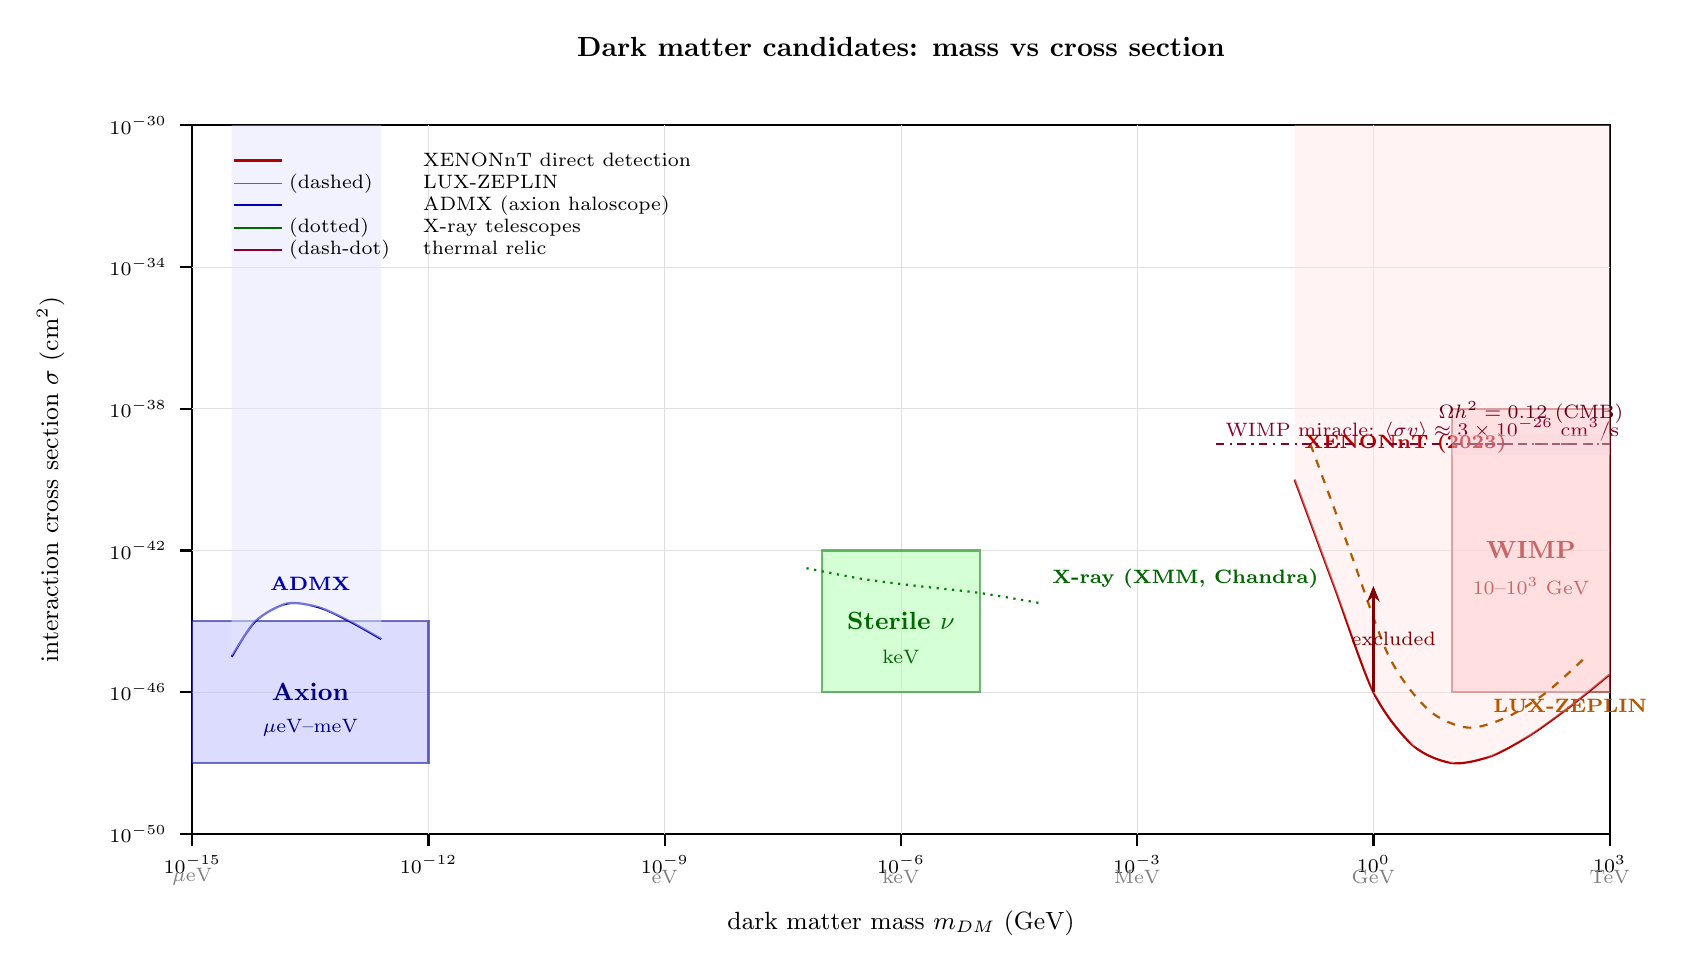
\begin{tikzpicture}[>={Stealth[length=2mm,width=1.6mm]}]

%================ Dark matter candidates: mass vs cross section ================
% X-axis: log10(m / GeV) from -15 (1 ueV) to +3 (1 TeV)
% Y-axis: log10(sigma / cm^2) from -50 to -30
% We use 1 unit = 1 decade
%
% Coordinate convention:
%   x = log10(m_DM / GeV)  ranges over [-15, 3]   -> width 18 units
%   y = log10(sigma / cm^2) ranges over [-50, -30] -> height 20 units, scaled by 0.45 -> 9 units high

\def\xmin{-15}
\def\xmax{3}
\def\ymin{-50}
\def\ymax{-30}
\def\ys{0.45}  % vertical scale: 1 decade -> 0.45 units

% Helper: macro to plot a (x, y) pair where x is log10 mass in GeV and y is log10 sigma
% TikZ axis area: x from \xmin to \xmax, y from \ymin*\ys to \ymax*\ys

% Title
\node[font=\bfseries] at ({(\xmin+\xmax)/2},{\ymax*\ys+1.0}) {Dark matter candidates: mass vs cross section};

% --- Draw axis box ---
\draw[thick,black] (\xmin,{\ymin*\ys}) rectangle (\xmax,{\ymax*\ys});

% --- X-axis ticks (every 3 decades) ---
\foreach \xv in {-15,-12,-9,-6,-3,0,3}{
  \draw[thick,black] (\xv,{\ymin*\ys}) -- (\xv,{\ymin*\ys-0.15});
  \node[font=\scriptsize,anchor=north] at (\xv,{\ymin*\ys-0.15}) {$10^{\xv}$};
}
\node[font=\small,anchor=north] at ({(\xmin+\xmax)/2},{\ymin*\ys-0.85})
  {dark matter mass $m_{DM}$ (GeV)};

% Mass scale labels above x-axis (ueV, eV, keV, MeV, GeV, TeV)
\node[font=\scriptsize,gray] at (-15,{\ymin*\ys-0.55}) {$\mu$eV};
\node[font=\scriptsize,gray] at (-9,{\ymin*\ys-0.55}) {eV};
\node[font=\scriptsize,gray] at (-6,{\ymin*\ys-0.55}) {keV};
\node[font=\scriptsize,gray] at (-3,{\ymin*\ys-0.55}) {MeV};
\node[font=\scriptsize,gray] at (0,{\ymin*\ys-0.55}) {GeV};
\node[font=\scriptsize,gray] at (3,{\ymin*\ys-0.55}) {TeV};

% --- Y-axis ticks (every 4 decades) ---
\foreach \yv in {-50,-46,-42,-38,-34,-30}{
  \draw[thick,black] (\xmin,{\yv*\ys}) -- (\xmin-0.15,{\yv*\ys});
  \node[font=\scriptsize,anchor=east] at (\xmin-0.2,{\yv*\ys}) {$10^{\yv}$};
}
\node[font=\small,rotate=90,anchor=south] at (\xmin-1.5,{(\ymin+\ymax)/2*\ys})
  {interaction cross section $\sigma$ (cm$^2$)};

% --- Light gridlines ---
\foreach \xv in {-12,-9,-6,-3,0}{
  \draw[gray!25,very thin] (\xv,{\ymin*\ys}) -- (\xv,{\ymax*\ys});
}
\foreach \yv in {-46,-42,-38,-34}{
  \draw[gray!25,very thin] (\xmin,{\yv*\ys}) -- (\xmax,{\yv*\ys});
}

%================ Candidate regions (filled, semi-transparent) ================

% --- Axion region: m ~ 10^-15 to 10^-12 GeV (1 ueV - 1 meV); sigma ~ 10^-48 to 10^-44 cm^2 ---
\fill[blue!25,opacity=0.55,draw=blue!60!black,thick]
  (-15,{-48*\ys}) rectangle (-12,{-44*\ys});
\node[font=\small\bfseries,blue!50!black] at (-13.5,{-46*\ys}) {Axion};
\node[font=\scriptsize,blue!50!black] at (-13.5,{-46*\ys-0.45}) {$\mu$eV--meV};

% --- Sterile neutrino region: m ~ 10^-6 GeV (keV scale); sigma ~ 10^-46 to 10^-42 cm^2 ---
\fill[green!30,opacity=0.55,draw=green!50!black,thick]
  (-7,{-46*\ys}) rectangle (-5,{-42*\ys});
\node[font=\small\bfseries,green!40!black] at (-6,{-44*\ys}) {Sterile $\nu$};
\node[font=\scriptsize,green!40!black] at (-6,{-44*\ys-0.45}) {keV};

% --- WIMP region: m ~ 10^1 to 10^3 GeV; sigma ~ 10^-46 to 10^-38 cm^2 ---
\fill[red!25,opacity=0.55,draw=red!60!black,thick]
  (1,{-46*\ys}) rectangle (3,{-38*\ys});
\node[font=\small\bfseries,red!60!black] at (2,{-42*\ys}) {WIMP};
\node[font=\scriptsize,red!60!black] at (2,{-42*\ys-0.45}) {10--$10^3$ GeV};

%================ Experimental exclusion contours ================

% --- XENONnT direct detection (2023): excludes WIMP region, m ~ 1 - 10^3 GeV
% Curve: shape of typical XENON spin-independent limit.
% Parametrise: minimum near m ~ 30-50 GeV at sigma ~ 10^-48; rises both sides.
% We draw a shaded "excluded above" region.
\draw[thick,red!70!black,smooth]
  plot coordinates {
    (-1.0,{-40*\ys})
    (-0.5,{-43*\ys})
    (0.0,{-46*\ys})
    (0.5,{-47.5*\ys})
    (1.0,{-48*\ys})
    (1.5,{-47.8*\ys})
    (2.0,{-47.2*\ys})
    (2.5,{-46.4*\ys})
    (3.0,{-45.5*\ys})
  };
% Fill the region above the XENON curve (excluded by direct detection)
\fill[red!10,opacity=0.45]
  plot coordinates {
    (-1.0,{-40*\ys})
    (-0.5,{-43*\ys})
    (0.0,{-46*\ys})
    (0.5,{-47.5*\ys})
    (1.0,{-48*\ys})
    (1.5,{-47.8*\ys})
    (2.0,{-47.2*\ys})
    (2.5,{-46.4*\ys})
    (3.0,{-45.5*\ys})
  } -- (3.0,{-30*\ys}) -- (-1.0,{-30*\ys}) -- cycle;
\node[font=\scriptsize\bfseries,red!70!black,anchor=west] at (-1.0,{-39*\ys}) {XENONnT (2023)};

% --- LUX-ZEPLIN exclusion (similar shape, slightly above XENON, dashed) ---
\draw[thick,dashed,orange!70!black,smooth]
  plot coordinates {
    (-0.8,{-39*\ys})
    (-0.3,{-42*\ys})
    (0.2,{-45*\ys})
    (0.7,{-46.5*\ys})
    (1.2,{-47*\ys})
    (1.7,{-46.7*\ys})
    (2.2,{-46.0*\ys})
    (2.7,{-45.0*\ys})
  };
\node[font=\scriptsize\bfseries,orange!70!black,anchor=west] at (1.4,{-46.4*\ys}) {LUX-ZEPLIN};

% --- ADMX axion haloscope: excludes a narrow band in axion region ---
\draw[thick,blue!70!black,smooth]
  plot coordinates {
    (-14.5,{-45*\ys})
    (-14.2,{-44*\ys})
    (-13.8,{-43.5*\ys})
    (-13.4,{-43.6*\ys})
    (-13.0,{-44*\ys})
    (-12.6,{-44.5*\ys})
  };
\fill[blue!10,opacity=0.5]
  plot coordinates {
    (-14.5,{-45*\ys})
    (-14.2,{-44*\ys})
    (-13.8,{-43.5*\ys})
    (-13.4,{-43.6*\ys})
    (-13.0,{-44*\ys})
    (-12.6,{-44.5*\ys})
  } -- (-12.6,{-30*\ys}) -- (-14.5,{-30*\ys}) -- cycle;
\node[font=\scriptsize\bfseries,blue!70!black,anchor=south] at (-13.5,{-43.4*\ys}) {ADMX};

% --- X-ray telescope (sterile neutrino decay): excludes upper part of sterile region ---
\draw[thick,green!50!black,smooth,dotted]
  plot coordinates {
    (-7.2,{-42.5*\ys})
    (-6.5,{-42.8*\ys})
    (-5.8,{-43.0*\ys})
    (-5.0,{-43.2*\ys})
    (-4.2,{-43.5*\ys})
  };
\node[font=\scriptsize\bfseries,green!40!black,anchor=west] at (-4.2,{-42.8*\ys}) {X-ray (XMM, Chandra)};

%================ Reference lines ================

% --- WIMP miracle thermal relic line: <sigma v> ~ 3e-26 cm^3/s
% Translating to a representative cross-section sigma ~ <sigma v>/v with v ~ 10^-3 c ~ 3e7 cm/s
% gives sigma ~ 10^-33 cm^2 (this is the annihilation-equivalent line)
% We draw a horizontal reference line and annotate
\draw[thick,dash dot,purple!70!black] (-2,{-39*\ys}) -- (3,{-39*\ys});
\node[font=\scriptsize,purple!70!black,anchor=west] at (-2,{-38.6*\ys})
  {WIMP miracle: $\langle\sigma v\rangle \approx 3\times 10^{-26}$ cm$^3$/s};

% --- Thermal relic band (Omega h^2 = 0.12) for WIMP region ---
\draw[thick,dashed,purple!50!black] (1,{-39*\ys}) -- (3,{-39*\ys});
\fill[purple!15,opacity=0.45] (1,{-39.3*\ys}) rectangle (3,{-38.7*\ys});
\node[font=\scriptsize,purple!50!black,anchor=south] at (2,{-38.7*\ys})
  {$\Omega h^2 = 0.12$ (CMB)};

%================ Legend ================
\node[anchor=north west,font=\scriptsize] at (\xmin+0.2,{\ymax*\ys-0.2})
  {\begin{tabular}{ll}
    \textcolor{red!70!black}{\rule[0.5ex]{0.6cm}{1pt}} & XENONnT direct detection \\
    \textcolor{orange!70!black}{\rule[0.5ex]{0.6cm}{0.6pt}} (dashed) & LUX-ZEPLIN \\
    \textcolor{blue!70!black}{\rule[0.5ex]{0.6cm}{1pt}} & ADMX (axion haloscope) \\
    \textcolor{green!40!black}{\rule[0.5ex]{0.6cm}{0.6pt}} (dotted) & X-ray telescopes \\
    \textcolor{purple!70!black}{\rule[0.5ex]{0.6cm}{0.6pt}} (dash-dot) & thermal relic \\
  \end{tabular}};

% --- Annotation arrows ---
% Show that thermal WIMP allowed window is being squeezed
\draw[->,thick,red!50!black] (0.0,{-46*\ys}) -- (0.0,{-43*\ys});
\node[font=\scriptsize,red!50!black,anchor=west] at (-0.4,{-44.5*\ys})
  {excluded};

\end{tikzpicture}
\end{document}
